% move all configuration stuff into one file so we can focus on the content
\documentclass[aspectratio=169,hyperref={pdfpagelabels=false,colorlinks=true,linkcolor=white,urlcolor=lightblue},xcolor={table},t]{beamer}

%%%%%%%%%%%%%%%%%%%%%%%%%%%%%%%%%%%%%%%%%%%%%%%%%%%%%%%%%%%%%%%%%%%%%%%%%%%%%%%%%%
%%%%%%%%%%%%%%%%%%%%%%%%%%%%%%%%%%%%%%%%%%%%%%%%%%%%%%%%%%%%%%%%%%%%%%%%%%%%%%%%%%
% packages
\usepackage{pict2e}
\usepackage{epic}
\usepackage{amsmath,amsfonts,amssymb}
\usepackage{units}
\usepackage{fancybox}
\usepackage[absolute,overlay]{textpos} 
%\usepackage[table]{xcolor}
\usepackage{animate}
\usepackage{gensymb}
%\usepackage{graphicx}
%\usepackage{longtable}
\usepackage{multirow}
\usepackage{silence}
\usepackage{tikz}
\usepackage[backend=bibtex,style=ieee]{biblatex}
\AtEveryCitekey{\iffootnote{\tiny}{}}
%\addbibresource{include/references}



% fontsize
\let\Tiny=\tiny

%%%%%%%%%%%%%%%%%%%%%%%%%%%%%%%%%%%%%%%%%%%%%%%%%%%%%%%%%%%%%%%%%%%%%%%%%%%%%%%%%%
%%%%%%%%%%%%%%%%%%%%%%%%%%%%%%%%%%%%%%%%%%%%%%%%%%%%%%%%%%%%%%%%%%%%%%%%%%%%%%%%%%
% warnings
\pdfsuppresswarningpagegroup=1
\WarningFilter{biblatex}{Patching footnotes failed}
\WarningFilter{latexfont}{Font shape}
\WarningFilter{latexfont}{Some font shapes}
\WarningFilter{gensymb}{Not defining}


%%%%%%%%%%%%%%%%%%%%%%%%%%%%%%%%%%%%%%%%%%%%%%%%%%%%%%%%%%%%%%%%%%%%%%%%%%%%%%%%%%
%%%%%%%%%%%%%%%%%%%%%%%%%%%%%%%%%%%%%%%%%%%%%%%%%%%%%%%%%%%%%%%%%%%%%%%%%%%%%%%%%%
% theme & layout
\usetheme{Frankfurt}
\useinnertheme{rectangles}


%%%%%%%%%%%%%%%%%%%%%%%%%%%%%%%%%%%%%%%%%%%%%%%%%%%%%%%%%%%%%%%%%%%%%%%%%%%%%%%%%%
\setbeamertemplate{frametitle}[default][colsep=-4bp,rounded=false,shadow=false]
\setbeamertemplate{frametitle}
{%
    \nointerlineskip%
    %\vskip-0.5ex
    \begin{beamercolorbox}[wd=\paperwidth,ht=3.5ex,dp=0.6ex]{frametitle}
        \hspace*{1.3ex}\insertframetitle%
        
        \hspace*{1.3ex}\small\insertframesubtitle%
    \end{beamercolorbox}%
    \begin{textblock*}{100mm}(13.75cm,1cm)
        
\includegraphics[height=.4cm,keepaspectratio]{../shared/Logo_GTCMT_white}
    \end{textblock*}
}


%%%%%%%%%%%%%%%%%%%%%%%%%%%%%%%%%%%%%%%%%%%%%%%%%%%%%%%%%%%%%%%%%%%%%%%%%%%%%%%%%%
\setbeamertemplate{title page}[default][colsep=-4bp,rounded=false,shadow=false]
\setbeamertemplate{title page}
{
    %\begin{textblock*}{100mm}(15cm,.51cm)
            %\href{https://github.com/alexanderlerch/ACA-Slides/blob/2nd_edition/\jobname.pdf}{\includegraphics[height=.5cm,keepaspectratio]{graph/Logo_github}}\hspace*{2ex}
    %\end{textblock*}
    %\begin{textblock*}{100mm}(15cm,1.3cm)
            %\href{\IEEELink}{\includegraphics[height=.5cm,keepaspectratio]{graph/icon/book}}\hspace*{2ex}
    %\end{textblock*}
    \vskip-10ex
    \begin{beamercolorbox}[wd=\paperwidth,ht=.7\paperheight,dp=0.6ex]{frametitle} %35ex
        %\begin{flushright}
            %\href{http://www.gtcmt.gatech.edu}{
\includegraphics[height=.8cm,keepaspectratio]{graph/Logo_GTCMT_black}}\hspace*{2ex}
        %\end{flushright}
        
        \hspace*{1.8ex}\LARGE\inserttitle%
        
        \vspace*{.5ex}
        
        \hspace*{1.3ex}\small\insertsubtitle%
        
        \vspace*{.5ex}
    \end{beamercolorbox}%
    \nointerlineskip%
    \begin{beamercolorbox}[wd=\paperwidth,ht=.4\paperheight,dp=0.6ex]{page number in head/foot}
        %\vspace*{-.5ex}
        \hspace*{1.7ex}\small\insertauthor%
        
        %\hspace*{1.7ex}\small }%
        
        \vspace*{12ex}
        \vfill
        \begin{flushright}
            \href{http://www.gtcmt.gatech.edu}{
\includegraphics[height=.5cm,keepaspectratio]{../shared/Logo_GTCMT_black}}\hspace*{2ex}
        \end{flushright}
    \end{beamercolorbox}%
}


%%%%%%%%%%%%%%%%%%%%%%%%%%%%%%%%%%%%%%%%%%%%%%%%%%%%%%%%%%%%%%%%%%%%%%%%%%%%%%%%%%
%\makeatother
\setbeamertemplate{footline}
{
  \leavevmode%
  \hbox{%
  \begin{beamercolorbox}[wd=.5\paperwidth,ht=2.25ex,dp=1ex,left,leftskip=1ex]{page number in head/foot}%
    \insertsubtitle
  \end{beamercolorbox}%
  \begin{beamercolorbox}[wd=.5\paperwidth,ht=2.25ex,dp=1ex,right,rightskip=1ex]{page number in head/foot}%
    \hfill
    \insertframenumber{} / \inserttotalframenumber
  \end{beamercolorbox}}%
  \vskip0pt%
}
%\makeatletter


%%%%%%%%%%%%%%%%%%%%%%%%%%%%%%%%%%%%%%%%%%%%%%%%%%%%%%%%%%%%%%%%%%%%%%%%%%%%%%%%%%
\beamertemplatenavigationsymbolsempty
\setbeamertemplate{navigation symbols}{}
\setbeamertemplate{blocks}[default]%[rounded=false,shadow=false]
\setbeamertemplate{itemize item}[square]
\setbeamertemplate{itemize subitem}[circle]
\setbeamertemplate{itemize subsubitem}[triangle]
\setbeamertemplate{enumerate item}[square]
\setbeamertemplate{enumerate subitem}[circle]
\setbeamertemplate{enumerate subsubitem}[circle]


%%%%%%%%%%%%%%%%%%%%%%%%%%%%%%%%%%%%%%%%%%%%%%%%%%%%%%%%%%%%%%%%%%%%%%%%%%%%%%%%%%
% colors
\setbeamercolor{structure}{fg=darkgray}
\setbeamercovered{transparent} %invisible
\setbeamercolor{bibliography entry author}{fg=black}
\setbeamercolor*{bibliography entry title}{fg=black}
\setbeamercolor*{bibliography entry note}{fg=black}
\setbeamercolor{frametitle}{fg=black}
\setbeamercolor{title}{fg=white}
\setbeamercolor{subtitle}{fg=white}
\setbeamercolor{frametitle}{fg=white}
\setbeamercolor{framesubtitle}{fg=white}
\setbeamercolor{mini frame}{fg=white, bg=black}
\setbeamercolor{section in head/foot}{fg=white, bg=darkgray}
\setbeamercolor{page number in head/foot}{fg=black, bg=gtgold}
\setbeamercolor{item projected}{fg=white, bg=black}

%---------------------------------------------------------------------------------

%%%%%%%%%%%%%%%%%%%%%%%%%%%%%%%%%%%%%%%%%%%%%%%%%%%%%%%%%%%%%%%%%%%%%%%%%%%%%%%%%%
%%%%%%%%%%%%%%%%%%%%%%%%%%%%%%%%%%%%%%%%%%%%%%%%%%%%%%%%%%%%%%%%%%%%%%%%%%%%%%%%%%
% title information
\title[]{MUSI6202: Digital Signal Processing for Music}   
\author[alexander lerch]{alexander lerch} 
%\institute{~}
%\date[Alexander Lerch]{}
%\titlegraphic{\vspace{-16mm}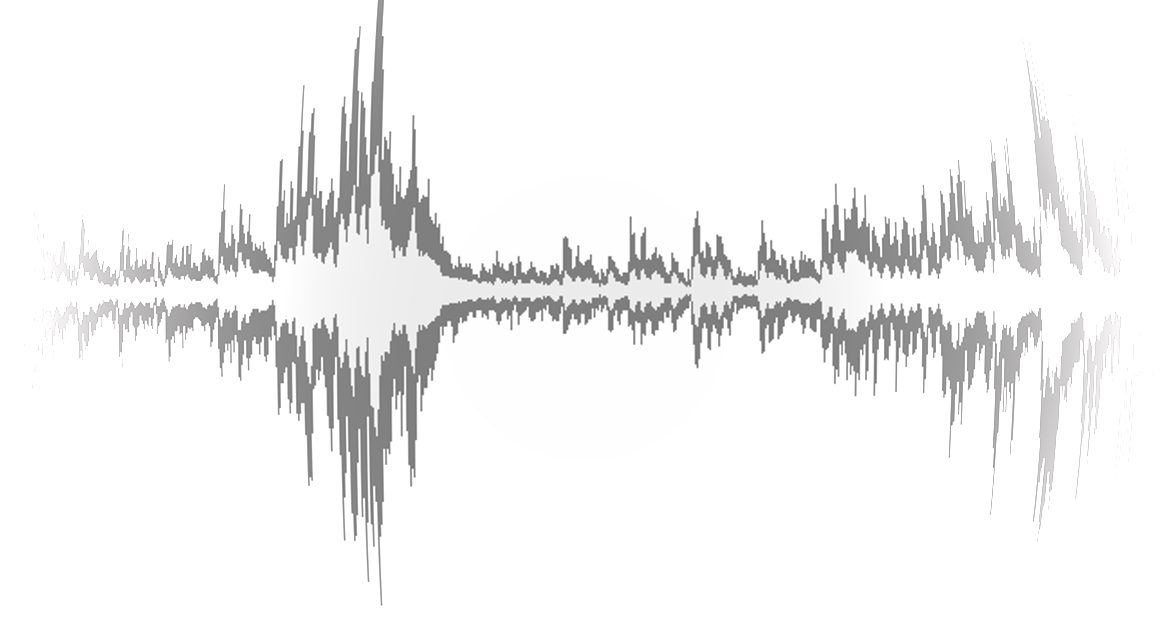
\includegraphics[width=\textwidth,height=3cm]{title}}

%%%%%%%%%%%%%%%%%%%%%%%%%%%%%%%%%%%%%%%%%%%%%%%%%%%%%%%%%%%%%%%%%%%%%%%%%%%%%%%%%%
%%%%%%%%%%%%%%%%%%%%%%%%%%%%%%%%%%%%%%%%%%%%%%%%%%%%%%%%%%%%%%%%%%%%%%%%%%%%%%%%%%
% colors
\definecolor{gtgold}{rgb}{.914, .664, 0} %0e7eed {rgb}{0.88,0.66,1,0.06} [234, 170, 0]/256 %96caff
\definecolor{darkgray}{rgb}{.15, .15, .15}
\definecolor{lightblue}{HTML}{0e7eed}
\definecolor{highlight}{rgb}{0, 0, 1} %_less!40

%%%%%%%%%%%%%%%%%%%%%%%%%%%%%%%%%%%%%%%%%%%%%%%%%%%%%%%%%%%%%%%%%%%%%%%%%%%%%%%%%%
%%%%%%%%%%%%%%%%%%%%%%%%%%%%%%%%%%%%%%%%%%%%%%%%%%%%%%%%%%%%%%%%%%%%%%%%%%%%%%%%%%
% relative paths
\graphicspath{{../graph/}}


%%%%%%%%%%%%%%%%%%%%%%%%%%%%%%%%%%%%%%%%%%%%%%%%%%%%%%%%%%%%%%%%%%%%%%%%%%%%%%%%%%
%%%%%%%%%%%%%%%%%%%%%%%%%%%%%%%%%%%%%%%%%%%%%%%%%%%%%%%%%%%%%%%%%%%%%%%%%%%%%%%%%%
% units
\setlength{\unitlength}{1mm}

%%%%%%%%%%%%%%%%%%%%%%%%%%%%%%%%%%%%%%%%%%%%%%%%%%%%%%%%%%%%%%%%%%%%%%%%%%%%%%%%%%
%%%%%%%%%%%%%%%%%%%%%%%%%%%%%%%%%%%%%%%%%%%%%%%%%%%%%%%%%%%%%%%%%%%%%%%%%%%%%%%%%%
% math
\DeclareMathOperator*{\argmax}{argmax}
\DeclareMathOperator*{\argmin}{argmin}
\DeclareMathOperator*{\atan}{atan}
\DeclareMathOperator*{\arcsinh}{arcsinh}
\DeclareMathOperator*{\sign}{sign}
\DeclareMathOperator*{\tcdf}{tcdf}
\DeclareMathOperator*{\si}{sinc}
\DeclareMathOperator*{\princarg}{princarg}
\DeclareMathOperator*{\arccosh}{arccosh}
\DeclareMathOperator*{\hwr}{HWR}
\DeclareMathOperator*{\flip}{flip}
\DeclareMathOperator*{\sinc}{sinc}
\DeclareMathOperator*{\floor}{floor}
\newcommand{\e}{{e}}
\newcommand{\jom}{\mathrm{j}\omega}
\newcommand{\jOm}{\mathrm{j}\Omega}
\newcommand   {\mat}[1]    		{\boldsymbol{\uppercase{#1}}}		%bold
\renewcommand {\vec}[1]    		{\boldsymbol{\lowercase{#1}}}		%bold

%%%%%%%%%%%%%%%%%%%%%%%%%%%%%%%%%%%%%%%%%%%%%%%%%%%%%%%%%%%%%%%%%%%%%%%%%%%%%%%%%%
%%%%%%%%%%%%%%%%%%%%%%%%%%%%%%%%%%%%%%%%%%%%%%%%%%%%%%%%%%%%%%%%%%%%%%%%%%%%%%%%%%
% media9
\newcommand{\includeaudio}[1]{
\href{run:audio/#1.mp3}{
\includegraphics[width=5mm, height=5mm]{graph/SpeakerIcon}}}

\newcommand{\includeanimation}[4]{{\begin{center}
                        \animategraphics[autoplay,loop,scale=.7]{#4}{animation/#1-}{#2}{#3}        
                        \end{center}
                        \addreference{matlab source: \href{https://github.com/alexanderlerch/ACA-Plots/blob/master/matlab/animate#1.m}{matlab/animate#1.m}}}
                        \inserticon{video}}
                        
%%%%%%%%%%%%%%%%%%%%%%%%%%%%%%%%%%%%%%%%%%%%%%%%%%%%%%%%%%%%%%%%%%%%%%%%%%%%%%%%%%
%%%%%%%%%%%%%%%%%%%%%%%%%%%%%%%%%%%%%%%%%%%%%%%%%%%%%%%%%%%%%%%%%%%%%%%%%%%%%%%%%%
% other commands
\newcommand{\question}[1]{%\vspace{-4mm}
                          \setbeamercovered{invisible}
                          \begin{columns}[T]
                            \column{.9\textwidth}
                                \textbf{#1}
                            \column{.1\textwidth}
                                \vspace{-8mm}
                                \begin{flushright}
                                     
\includegraphics[width=.9\columnwidth]{graph/question_mark}
                                \end{flushright}
                                \vspace{6mm}
                          \end{columns}\pause\vspace{-12mm}}

\newcommand{\toremember}[1]{
                        \inserticon{lightbulb}
                        }

\newcommand{\matlabexercise}[1]{%\vspace{-4mm}
                          \setbeamercovered{invisible}
                          \begin{columns}[T]
                            \column{.8\textwidth}
                                \textbf{matlab exercise}: #1
                            \column{.2\textwidth}
                                \begin{flushright}
                                     \includegraphics[scale=.5]{graph/logo_matlab}
                                \end{flushright}
                                %\vspace{6mm}
                          \end{columns}}

\newcommand{\addreference}[1]{  
                  
                    \begin{textblock*}{\baselineskip }(.98\paperwidth,.5\textheight) %(1.15\textwidth,.4\textheight)
                         \begin{minipage}[b][.5\paperheight][b]{1cm}%
                            \vfill%
                             \rotatebox{90}{\tiny {#1}}
                        \end{minipage}
                   \end{textblock*}
                    }
                    
\newcommand{\figwithmatlab}[1]{
                    \begin{figure}
                        \centering
                        \includegraphics[scale=.7]{#1}
                        %\label{fig:#1}
                    \end{figure}
                    
                    \addreference{matlab source: \href{https://github.com/alexanderlerch/MUSI-6202/blob/main/matlab/plot#1.m}{plot#1.m}}}
\newcommand{\figwithref}[2]{
                    \begin{figure}
                        \centering
                        \includegraphics[scale=.7]{#1}
                        \label{fig:#1}
                    \end{figure}
                    
                    \addreference{#2}}  
                                    
\newcommand{\inserticon}[1]{
                    \begin{textblock*}{100mm}(14.5cm,7.5cm)
                        \includegraphics[height=.8cm,keepaspectratio]{graph/#1}
                    \end{textblock*}}            

%%%%%%%%%%%%%%%%%%%%%%%%%%%%%%%%%%%%%%%%%%%%%%%%%%%%%%%%%%%%%%%%%%%%%%%%%%%%%%%%%%
%%%%%%%%%%%%%%%%%%%%%%%%%%%%%%%%%%%%%%%%%%%%%%%%%%%%%%%%%%%%%%%%%%%%%%%%%%%%%%%%%%
% counters
\newcounter{i}
\newcounter{j}
\newcounter{iXOffset}
\newcounter{iYOffset}
\newcounter{iXBlockSize}
\newcounter{iYBlockSize}
\newcounter{iYBlockSizeDiv2}
\newcounter{iXBlockSizeDiv2}
\newcounter{iDistance}

\newcommand{\IEEELink}{https://ieeexplore.ieee.org/servlet/opac?bknumber=9965970}

\addbibresource{../shared/references}



\subtitle{Part 26: Perceptual Coding}

%%%%%%%%%%%%%%%%%%%%%%%%%%%%%%%%%%%%%%%%%%%%%%%%%%%%%%%%%%%%%%%%%%%%%%%%%%%%
\begin{document}
    % generate title page
	\title[]{Digital Signal Processing for Music}   
\author[alexander lerch]{alexander lerch} 
%\institute{~}
%\date[Alexander Lerch]{}
\titlegraphic{\vspace{-16mm}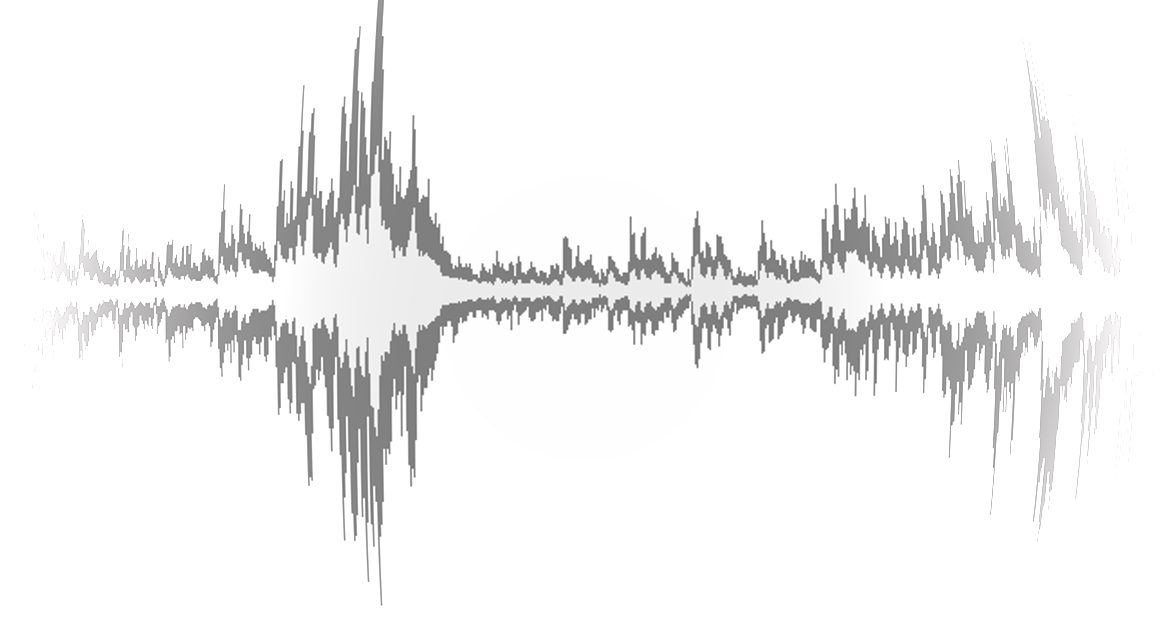
\includegraphics[width=\textwidth,height=3cm]{title}}


\begin{frame}
    \titlepage
    %\vspace{-5mm}
    \begin{flushright}
        \href{http://www.gtcmt.gatech.edu}{
\includegraphics[height=.8cm,keepaspectratio]{../shared/Logo_GTCMT_black}}
    \end{flushright}
\end{frame}


\section[intro]{introduction}

	\begin{frame}{perceptual coding}{introduction}
        \begin{itemize}
            \item   \textbf{goal}: 
                \begin{itemize}
                    \item   encode signal in a way that the decoded signal is \textbf{perceptually} as close to the original signal as possible
                \end{itemize}
            \pause
            \bigskip
            \item   \textbf{common codecs}:
                \begin{itemize}
                    \item   MPEG-1/2 Layer 2
                    \item   MPEG-1/2 Layer 3
                    \item   %\color<5->{gtgold}{
                    MPEG-2/4 AAC
                    \item   AC-3/4
                    \item   Ogg Vorbis
                    \item   (DTS  Cine/Home)
                    \item   (ATRAC)
                \end{itemize}
        \end{itemize}
	\end{frame}
	\begin{frame}{perceptual coding}{brainstorming}
        \question{how do we detect and remove perceptually irrelevant information}
        
        \begin{enumerate}
            \item   build a perceptual (psycho-acoustic) model and utilize insights on physiological and cognitive properties of average human's sound reception
            \bigskip
            \item   quantize identified irrelevant components more aggressively than important components
        \end{enumerate}
	\end{frame}
	\begin{frame}{perceptual coding}{overview}
        \vspace{-5mm}
        \begin{figure}
			\begin{center}
	            \begin{picture}(90,70)
	
	                %boxes \colorbox{gray!20}
	                \put(0,40){\framebox (20,10){\scriptsize\color<2>{gtgold}\shortstack[c]{Psychoacoustic\\ Model}}}
	                \put(0,0){\framebox (20,10){\scriptsize\shortstack[c]{Bit Allocation}}}

	                \put(30,40){\framebox (20,10){\scriptsize\shortstack[c]{Frequency\\ Transformation}}}
	                \put(30,20){\framebox (20,10){\scriptsize\shortstack[c]{Additional\\ Processing}}}
	                \put(30,0){\framebox (20,10){\scriptsize\shortstack[c]{Quantization\\ Entropy Coding}}}
	
	                \put(60,0){\framebox (20,50){\scriptsize\shortstack[c]{Bitstream\\ Formatting}}}

	                %lines horizontal
	                \put(10,25){\vector(1,0){20}}
	                \put(20,5){\vector(1,0){10}}
	                \put(10,60){\line(1,0){30}}

	                \put(50,45){\vector(1,0){10}}
	                \put(50,25){\vector(1,0){10}}
	                \put(50, 5){\vector(1,0){10}}

	                \put(80,25){\vector(1,0){5}}
	
	                %lines vertical
	                \put(10,60){\vector(0,-1){10}}
	                \put(10,40){\vector(0,-1){30}}

	                \put(40,65){\vector(0,-1){15}}
	                \put(40,40){\vector(0,-1){10}}
	                \put(40,20){\vector(0,-1){10}}
	                
	                %circles
	                \put(10,25){\circle*{1}}

	                \put(40,60){\circle*{1}}
	
	                %text
	                \put(42,65){\footnotesize{\shortstack[c]{input}}}
	                \put(84,27){\footnotesize{\shortstack[c]{bitstream}}}
	            \end{picture}
			\end{center}
	    \end{figure}
	\end{frame}
    
	\section[psycho]{psychoacoustic model}
	\begin{frame}{source coding}{psycho-acoustic model: overview}
        \begin{itemize}
            \item   \textbf{objective}:\\ identify components perceptible and imperceptible by humans
            \pause
            \smallskip
            \item   \textbf{approach}:\\ build model of human sound perception (\textit{analysis only!})
            \pause
            \smallskip
            \item   \textbf{processing steps}:
                \begin{enumerate}
                    \item	transform to \textbf{frequency domain}
                    \pause
                    \item	map to \textbf{perceptual frequency scale}
                    \pause
                    \item   group into bands
                    \pause
                    \item	compute (perceptual) \textbf{masking threshold}
                    \pause
                    \item	compute \textbf{Signal-to-Mask Ratio} (SMR)
                    \pause
                    \item   compute additional analysis results
                \end{enumerate}
            \pause
            \smallskip
            \item   \textbf{recommendation only}! no standardization of implementation
        \end{itemize}
	\end{frame}
	
	\begin{frame}{source coding}{psycho-acoustic model 1--3: frequency transform}
        %\vspace{-3mm}
		\begin{enumerate}
            \item   frequency transformation (AAC: FFT)
            \item   frequency warping (AAC: Bark scale)
            \item   group power in bands (AAC: \nicefrac{1}{3} Bark resolution)
        \end{enumerate}
            \begin{figure}
				\centering
					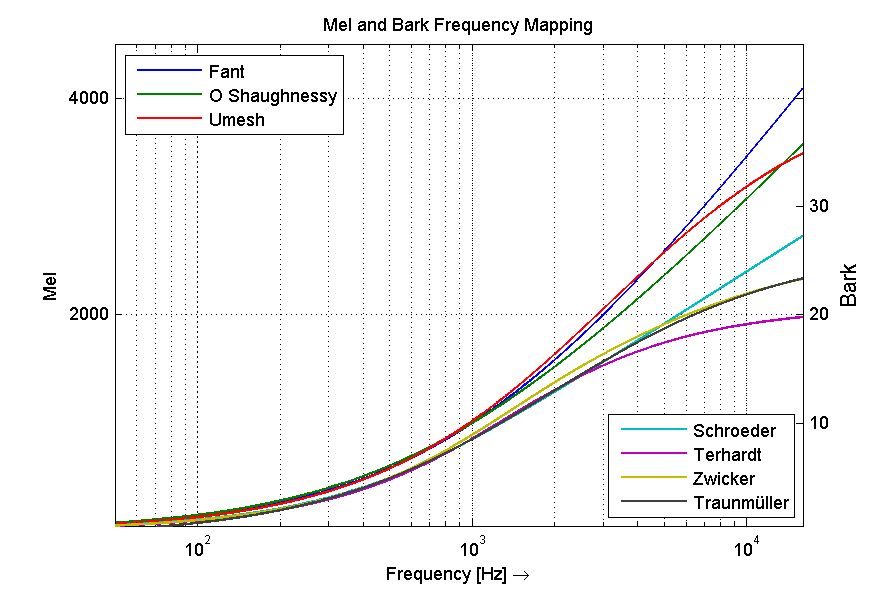
\includegraphics[scale=0.5]{Graph/mel}
			\end{figure}
	\end{frame}
	
	\begin{frame}{source coding}{psycho-acoustic model 4: masking threshold 1/2}
        \begin{itemize}
            \item   humans are not able to perceive every possible detail in an audio signal
                \begin{enumerate}[i]
                    \item<1->   frequency resolution (see above)
                    \item<1->   sensitivity for specific frequency regions
                        \only<1>{
                        \begin{figure}
                            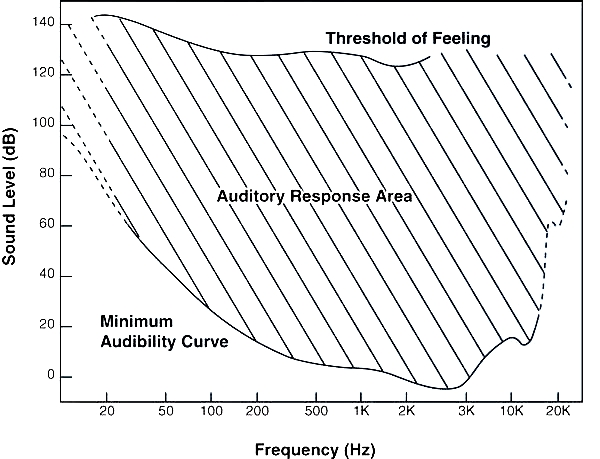
\includegraphics[scale=.25]{graph/hearingarea}
                        \end{figure}}
                    \item<2->   components masked by other components
                         \only<2>{
                        \begin{figure}
                            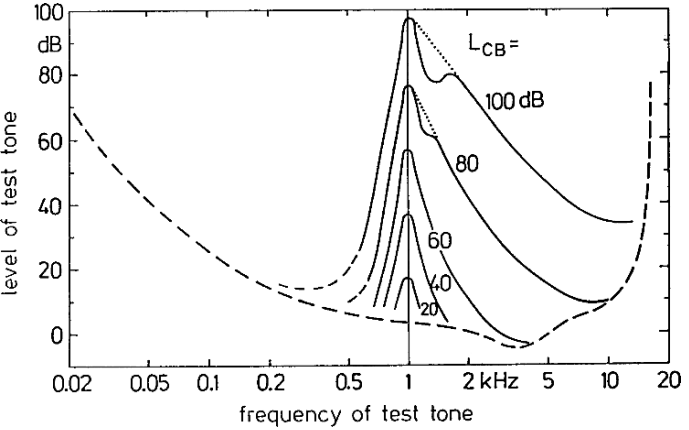
\includegraphics[scale=.25]{graph/maskingtonebynarrownoise2}
                            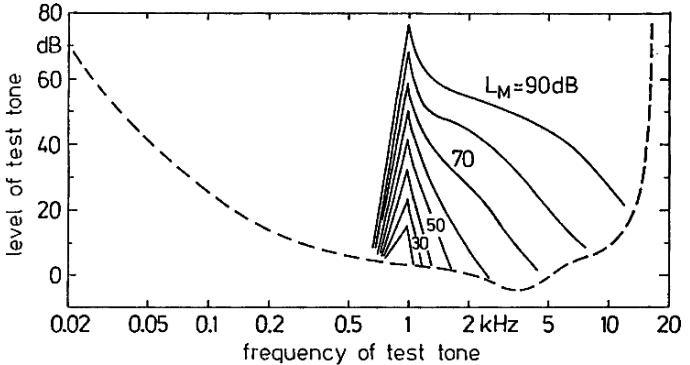
\includegraphics[scale=.25]{graph/maskingtonebytone}
                            
                            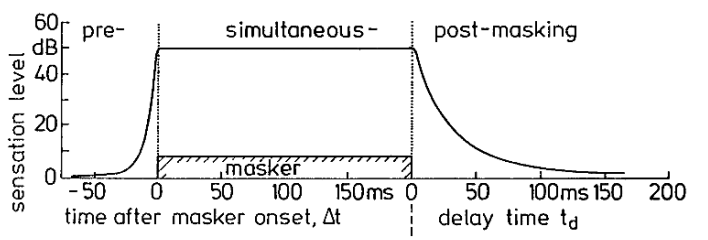
\includegraphics[scale=.25]{graph/maskingtemporal}
                        \end{figure}}
                    \item<3->   masking threshold depends on
                            \begin{itemize}
                                \item   \textit{frequency} of masker
                                \item   \textit{noisiness} of masker
                                \item   \textit{level} of masker
                                \item   \textit{duration} of masker
                            \end{itemize}
               \end{enumerate}
        \end{itemize}
        \vspace{70mm}
	\end{frame}
	
	\begin{frame}{source coding}{psycho-acoustic model 4: masking threshold 2/2}
        AAC computation of masking threshold (recommendation)
        \begin{itemize}
            \item       take hearing threshold as minimum masking threshold
            \item<2->   convolve band spectrum with spreading function
                        \uncover<2->
                        {
                        \begin{figure}
                            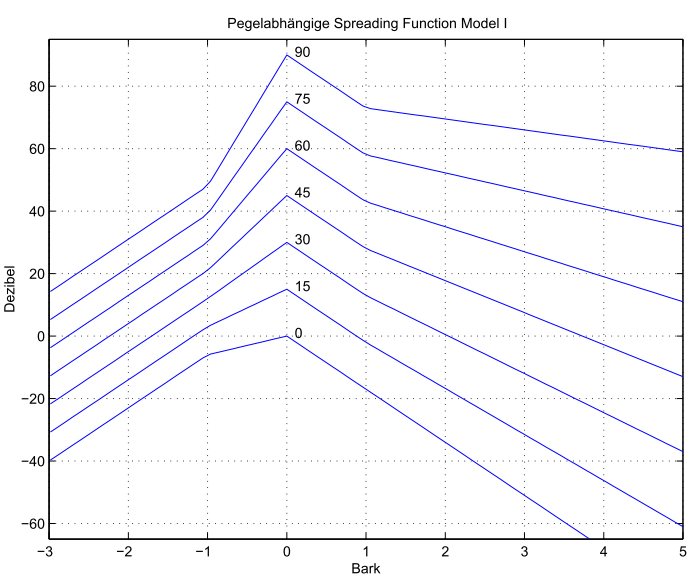
\includegraphics[scale=.25]{graph/spreadingfunction_layer2}
                            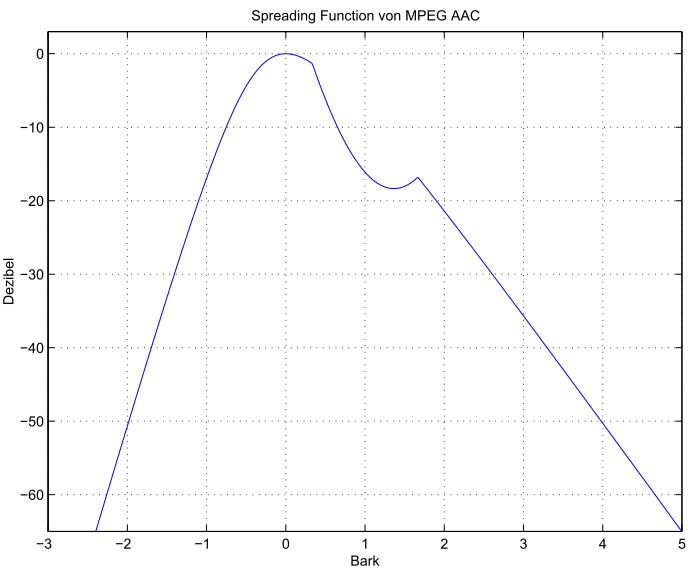
\includegraphics[scale=.25]{graph/spreadingfunction_aac}
                        \end{figure}}
            \item<3->   compute tonality (with phase deviation) and apply to masking threshold (from original spectrum)
        \end{itemize}
        
	\end{frame}
	
	\begin{frame}{source coding}{psycho-acoustic model: visualization}
		\vspace{-4mm}	
        \begin{figure}
				\centering
					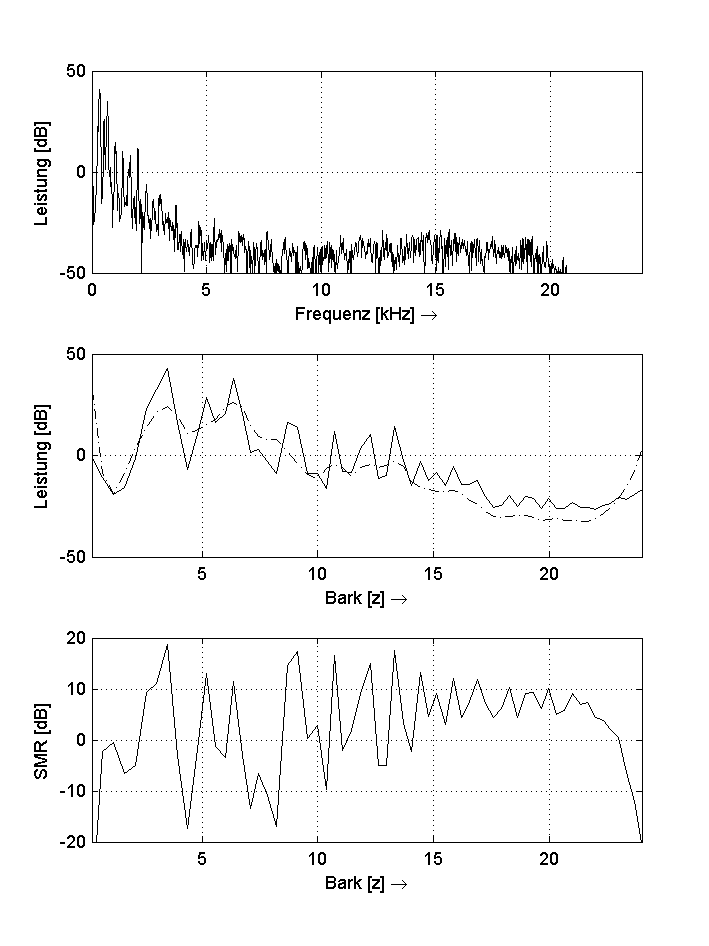
\includegraphics[scale=0.4]{Graph/Lerch16-8}
					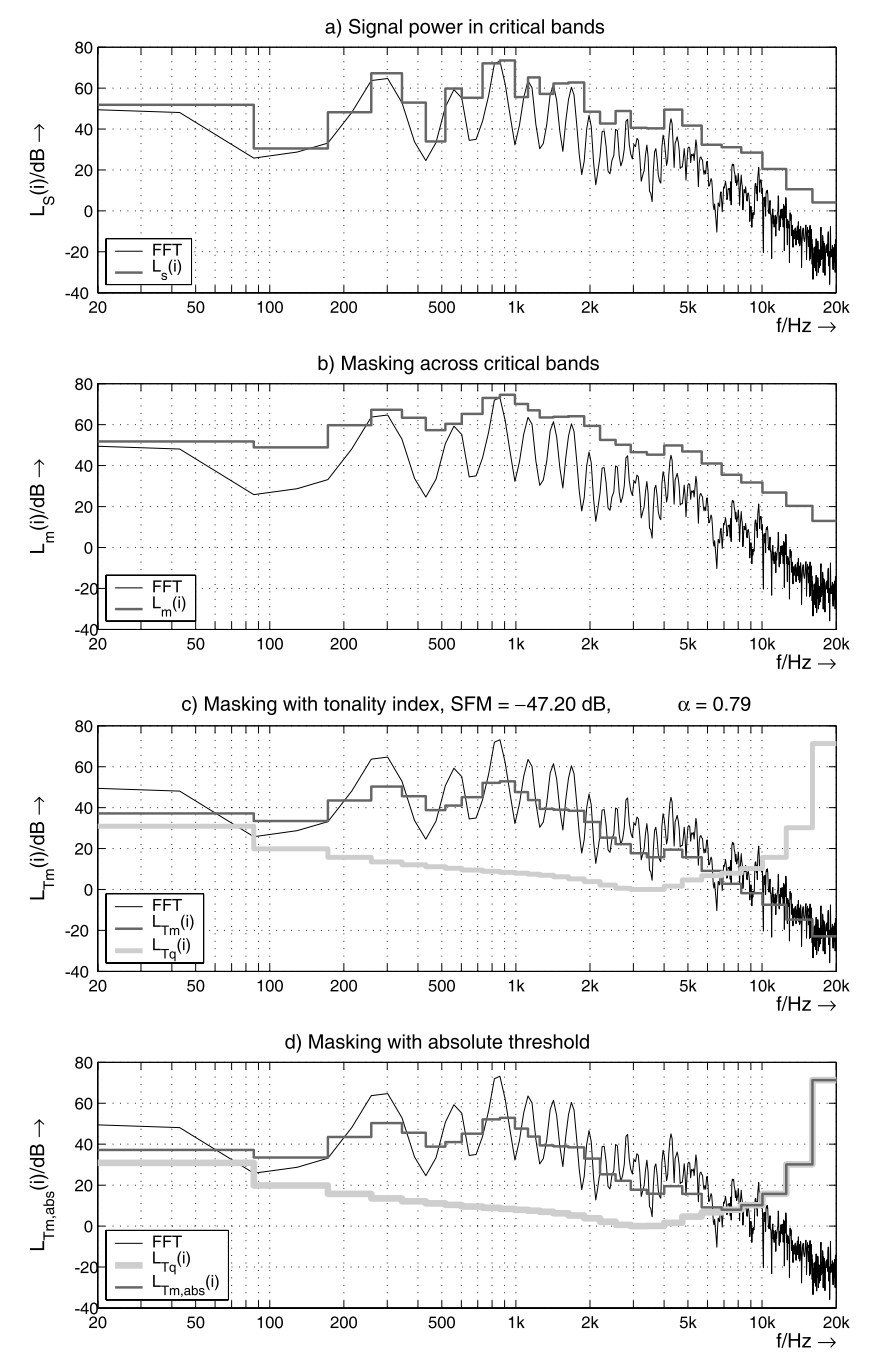
\includegraphics[scale=0.2]{Graph/psychomodeloutput}
			\end{figure}
	\end{frame}
	
	\begin{frame}{source coding}{psycho-acoustic model: additionally extracted information}
        \begin{itemize}
            \item   in addition to Signal-to-Mask ratio, psycho-acoustic model may output other control outputs, e.g., for
                \begin{itemize}
                    \item   \textbf{bit reservoir} 
                    \smallskip
                    \item \textbf{window length switching}
                    \smallskip
                    \item   \textbf{joint stereo parameters}
                \end{itemize}
        \end{itemize}
	\end{frame}
    \section[quantization]{quantization \& entropy coding}
	\begin{frame}{perceptual coding}{overview}
        \vspace{-5mm}
        \begin{figure}
			\begin{center}
	            \begin{picture}(90,70)
	
	                %boxes \colorbox{gray!20}
	                \put(0,40){\framebox (20,10){\scriptsize\shortstack[c]{Psychoacoustic\\ Model}}}
	                \put(0,0){\framebox (20,10){\scriptsize\color<1>{gtgold}\shortstack[c]{Bit Allocation}}}

	                \put(30,40){\framebox (20,10){\scriptsize\shortstack[c]{Frequency\\ Transformation}}}
	                \put(30,20){\framebox (20,10){\scriptsize\shortstack[c]{Additional\\ Processing}}}
	                \put(30,0){\framebox (20,10){\scriptsize\color<1>{gtgold}\shortstack[c]{Quantization\\ Entropy Coding}}}
	
	                \put(60,0){\framebox (20,50){\scriptsize\shortstack[c]{Bitstream\\ Formatting}}}

	                %lines horizontal
	                \put(10,25){\vector(1,0){20}}
	                \put(20,5){\vector(1,0){10}}
	                \put(10,60){\line(1,0){30}}

	                \put(50,45){\vector(1,0){10}}
	                \put(50,25){\vector(1,0){10}}
	                \put(50, 5){\vector(1,0){10}}

	                \put(80,25){\vector(1,0){5}}
	
	                %lines vertical
	                \put(10,60){\vector(0,-1){10}}
	                \put(10,40){\vector(0,-1){30}}

	                \put(40,65){\vector(0,-1){15}}
	                \put(40,40){\vector(0,-1){10}}
	                \put(40,20){\vector(0,-1){10}}
	                
	                %circles
	                \put(10,25){\circle*{1}}

	                \put(40,60){\circle*{1}}
	
	                %text
	                \put(42,65){\footnotesize{\shortstack[c]{input}}}
	                \put(84,27){\footnotesize{\shortstack[c]{bitstream}}}
	            \end{picture}
			\end{center}
	    \end{figure}
	\end{frame}
	
	\begin{frame}{perceptual coding}{bit allocation}
        \begin{itemize}
            \item   \textbf{goal}
            \begin{itemize}
                \item   intelligently distribute available bits over bands 
            \end{itemize}
            \bigskip
            \item<2->   \textbf{optimization problem}:
                \begin{itemize}
                    \item   psycho-acoustic model indicates how many bits are \textbf{required} (SMR)
                    \smallskip
                    \item   user settings indicate how many bits are \textbf{available} per block
                    \smallskip
                    \item   actual number of encoded bits is unclear (\textbf{entropy coding}!)
                \end{itemize}
            \bigskip
            \item<3->   advanced encoders might iterate over trial encodings
        \end{itemize}
	\end{frame}
	
	\begin{frame}{perceptual coding}{bit reservoir}
        \vspace{-3mm}
		\begin{itemize}
			\item	constant bitrate per frame puts tight constraints on encoder as some blocks are easier to encode than others
            \bigskip
            \item<2->[$\Rightarrow$] \textbf{bit reservoir}
                \begin{itemize}
                    \item utilize 'unused' bits in easy to encode frames for extra bits for difficult to encode frames
                \end{itemize}
		\end{itemize}
        \vspace{-5mm}
        \begin{columns}
        \column{.65\linewidth}
		\begin{itemize}
            \item implementation
				\begin{itemize}
					\item	allocate extra bits for bit reservoir ($\approx 6000 bits$, bit rate dependent)
                        \begin{itemize}
                            \item   actual rate must never exceed channel capacity
                            \item   some frames might need more bits to properly encode
                            \item   allow deviation from constant bitrate at the cost of latency
                            \item   has to be allocated from previous frames 
                            \item   causes additional decoder delay/latency
                        \end{itemize}
				\end{itemize}
		\end{itemize}
        \column{.35\linewidth}
                        \begin{figure}
                            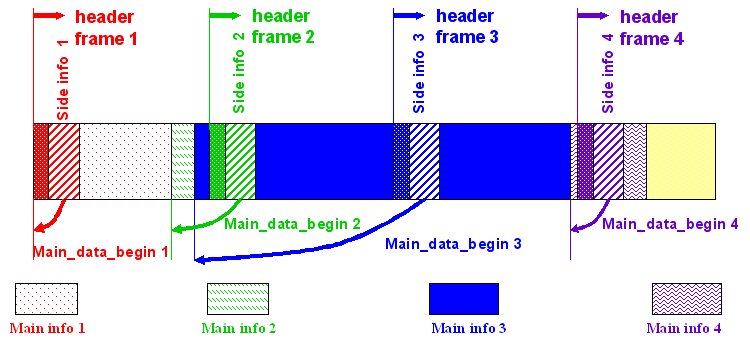
\includegraphics[scale=.2]{graph/bit_reservoir}
                        \end{figure}
        \end{columns}
	\end{frame}
	
	\begin{frame}{perceptual coding}{quantization \& entropy coding}
		\begin{itemize}
			\item	\textbf{quantization}
				\begin{itemize}
					\item	re-quantize the spectrum per band
					\item	each band has different \textit{scaling factor} and \textit{word length}
                    \item   non-uniform quantization
				\end{itemize}
			\pause
			\bigskip
            \item	\textbf{entropy coding}
				\begin{itemize}
					\item	apply lossless coding (multiple dictionaries)
					\item	submit the gained bits to bit allocation (re-iterate?)
				\end{itemize}
		\end{itemize}
	\end{frame}

\section[artifacts]{artifacts \& tweaks}	
	\begin{frame}{perceptual coding}{artifacts: transient smearing and pre-echo}
		\begin{itemize}
			\item	\textbf{transient smearing}\\
					transients are smoothed out
			\smallskip
            \item	\textbf{musical noise} (ringing, birdies)\\
					switch high frequency bands on and off
			\smallskip
            \item	\textbf{stereo imaging}\\
					changing localization and spatial impression
			\smallskip
            \item	\textbf{roughness}\\
					time-variant granular quantization noise
		\end{itemize}
	\end{frame}
	\begin{frame}{perceptual coding}{artifacts: transient smearing and pre-echo}
			\begin{figure}
				\centering
					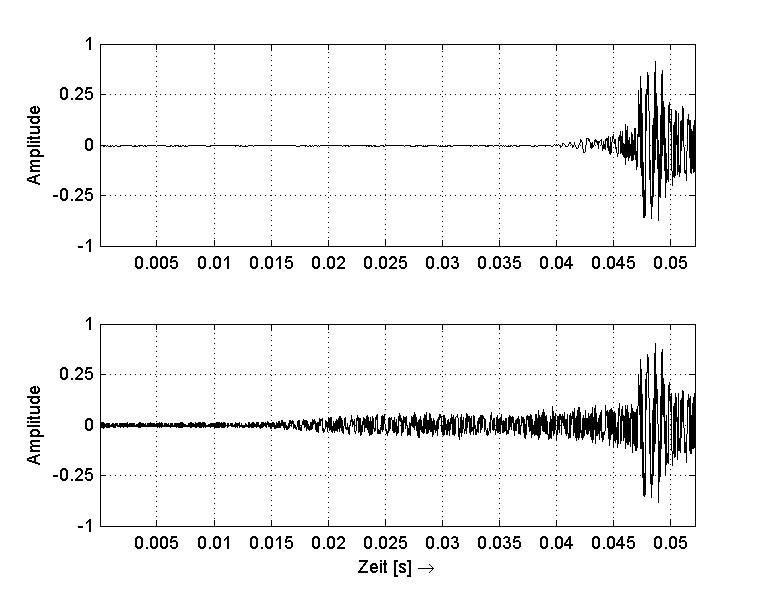
\includegraphics[scale=0.5]{Graph/Lerch16-9}
			\end{figure}
	\end{frame}
	
\section[tweaks]{AAC tools}	
	\begin{frame}{perceptual coding}{overview}
        \vspace{-5mm}
        \begin{figure}
			\begin{center}
	            \begin{picture}(90,70)
	
	                %boxes \colorbox{gray!20}
	                \put(0,40){\framebox (20,10){\scriptsize\shortstack[c]{Psychoacoustic\\ Model}}}
	                \put(0,0){\framebox (20,10){\scriptsize\shortstack[c]{Bit Allocation}}}

	                \put(30,40){\framebox (20,10){\scriptsize\shortstack[c]{Frequency\\ Transformation}}}
	                \put(30,20){\framebox (20,10){\scriptsize\color<1>{gtgold}\shortstack[c]{Additional\\ Processing}}}
	                \put(30,0){\framebox (20,10){\scriptsize\shortstack[c]{Quantization\\ Entropy Coding}}}
	
	                \put(60,0){\framebox (20,50){\scriptsize\shortstack[c]{Bitstream\\ Formatting}}}

	                %lines horizontal
	                \put(10,25){\vector(1,0){20}}
	                \put(20,5){\vector(1,0){10}}
	                \put(10,60){\line(1,0){30}}

	                \put(50,45){\vector(1,0){10}}
	                \put(50,25){\vector(1,0){10}}
	                \put(50, 5){\vector(1,0){10}}

	                \put(80,25){\vector(1,0){5}}
	
	                %lines vertical
	                \put(10,60){\vector(0,-1){10}}
	                \put(10,40){\vector(0,-1){30}}

	                \put(40,65){\vector(0,-1){15}}
	                \put(40,40){\vector(0,-1){10}}
	                \put(40,20){\vector(0,-1){10}}
	                
	                %circles
	                \put(10,25){\circle*{1}}

	                \put(40,60){\circle*{1}}
	
	                %text
	                \put(42,65){\footnotesize{\shortstack[c]{input}}}
	                \put(84,27){\footnotesize{\shortstack[c]{bitstream}}}
	            \end{picture}
			\end{center}
	    \end{figure}
	\end{frame}
	\begin{frame}{perceptual coding}{tweaks: block switching}
			\begin{figure}
				\centering
					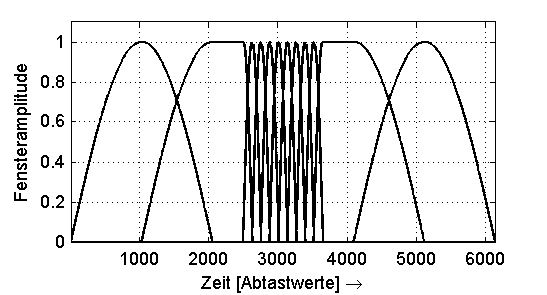
\includegraphics[scale=0.9]{Graph/Lerch16-4}
			\end{figure}
            \begin{itemize}
                \item   AAC: transients are encoded by 8 short frames (256) instead of 1 long frame (2048)
                \item   introduces additional encoding delay because of different start window shape
            \end{itemize}
	\end{frame}
    
	
	\begin{frame}{perceptual coding}{tweaks: other tools (MPEG-4 AAC, 1st generation) 1/2}
		\begin{itemize}
			\item	\textbf{joint stereo coding}
                \begin{itemize}
                    \item   MS (mid/side stereo)
                        \begin{itemize}
                            \item   exploit inter-channel \textit{redundancy} by Mid/Side encoding
                        \end{itemize}
                    \item   IS (intensity stereo)
                        \begin{itemize}
                            \item   remove \textit{irrelevancy} of stereo information: replace stereo by one signal with directional information
                            \item   works for high frequencies (per band)
                            \item   may result in spatial distortions
                        \end{itemize}
                \end{itemize}
            \pause
            \bigskip
            
            \item   \textbf{prediction}
                \begin{itemize}
                    \item   FDP (frequency domain prediction)
                        \begin{itemize}
                            \item   backward adaptive per band
                            \item   increases decoder complexity
                        \end{itemize}
                    \item   LTP (long term prediction)
                        \begin{itemize}
                            \item   time domain prediction, forward adaptive, one coefficient, large lag
                        \end{itemize}
                \end{itemize}
		\end{itemize}
	\end{frame}
    \begin{frame}{perceptual coding}{tweaks: other tools (MPEG-4 AAC, 1st generation) 2/2}
		\begin{itemize}
		\item	\textbf{TNS} (temporal noise shaping)
                \begin{itemize}
                    \item   transient artifacts remain problematic
                    \item   D$^\ast$PCM in the frequency domain $\rightarrow$ time-domain envelope of the error shaped after signal envelope
                    \item[$\Rightarrow$] shift quantization error power to high amplitude regions!
                \end{itemize}
            \begin{figure}
                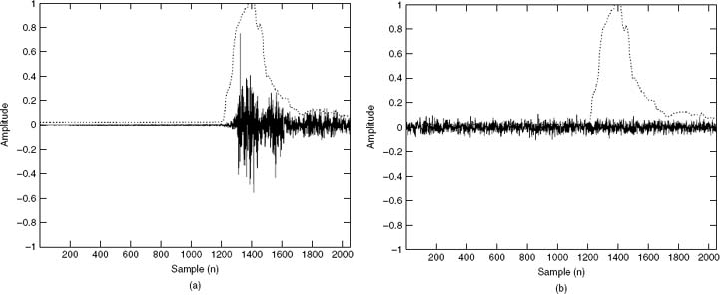
\includegraphics[scale=.6]{graph/tns.png}
            \end{figure}
			\pause
            \bigskip
            \item	\textbf{PNS} (perceptual noise substitution)
                \begin{itemize}
                    \item   transmit noise level and inter-channel correlation instead of encoding noise subbands
                \end{itemize}
		\end{itemize}
	\end{frame}
    \begin{frame}{perceptual coding}{tweaks: other tools (MPEG-4 AAC, 2nd generation) 1/2}
        \begin{itemize}
			\item	\textbf{PS} (parametric stereo)
                \begin{itemize}
                    \item   extends the IS concept:
                    \item[] encode \textit{one} channel and transmit control info to generate the other channel
                \end{itemize}
		\end{itemize}
	\end{frame}
    \begin{frame}{perceptual coding}{tweaks: other tools (MPEG-4 AAC, 2nd generation) 2/2}
        \vspace{-3mm}
        \begin{itemize}
            \item	\textbf{SBR} (spectral band replication)
                \begin{itemize}
                    \item encode \textit{band limited} signal and transmit control info to generate high frequency content
                \end{itemize}
		\end{itemize}
        \begin{figure}
            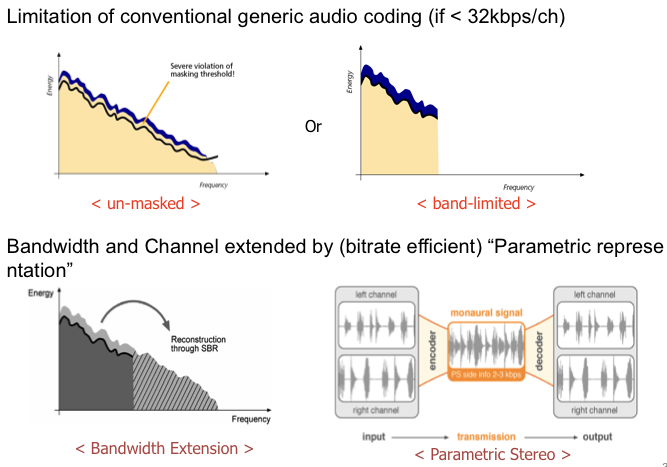
\includegraphics[scale=.5]{graph/sbr}
        \end{figure}
	\end{frame}
	
	\begin{frame}{perceptual coding}{artifacts reminder}
		\begin{itemize}
			\item	\textbf{transient smearing}\\
					transients are smoothed out
			\smallskip
            \item	\textbf{musical noise} (ringing)\\
					switch high frequency bands on and off
			\smallskip
            \item	\textbf{stereo imaging}\\
					changing localization and spatial impression
			\smallskip
            \item	\textbf{roughness}\\
					time-variant granular quantization noise
		\end{itemize}
	\end{frame}

\section[audio]{audio examples}	
	\begin{frame}{perceptual coding}{audio examples (MP3)}
        \begin{columns}
            \column{.5\textwidth}
            \textbf{Harspichord}
                \begin{itemize}
                    \item   original \includeaudio{mp3Original}
                    \item   \unit[256]{kbps} \includeaudio{mp3_256}
                    \item   \unit[128]{kbps} \includeaudio{mp3_128}
                    \item   \unit[96]{kbps} \includeaudio{mp3_96}
                    \item   \unit[64]{kbps} \includeaudio{mp3_64}
                    \item   \unit[32]{kbps} \includeaudio{mp3_32}
                \end{itemize}
            \column{.5\textwidth}
            \textbf{Percussion}
                \begin{itemize}
                    \item   original \includeaudio{Mp3_Perc_original}
                    \item   \unit[256]{kbps} \includeaudio{Mp3_Perc_256}
                    \item   \unit[128]{kbps} \includeaudio{Mp3_Perc_128}
                    \item   \unit[96]{kbps} \includeaudio{Mp3_Perc_96}
                    \item   \unit[64]{kbps} \includeaudio{Mp3_Perc_64}
                    \item   \unit[32]{kbps} \includeaudio{Mp3_Perc_32}
                \end{itemize}
        \end{columns}
	\end{frame}

\section{bitrate models}	
	\begin{frame}{perceptual coding}{bitrate models}
		\begin{itemize}	
			\item	\textbf{constant bit rate} (CBR):
					\begin{itemize}
						\item	bit rate constant over time
						\item	quality changes over time
					\end{itemize}
			\bigskip
            \item	\textbf{variable bit rate} (VBR):
					\begin{itemize}
						\item	bit rate changes over time
						\item	quality constant over time (depends on psychoacoustic model)
					\end{itemize}
		\end{itemize}
	\end{frame}		

\section[codecs]{codec overview}
	\begin{frame}{perceptual coding}{algorithms \& properties}
		\begin{table}
			\begin{center}
			\begin{footnotesize}
				\begin{tabular}{lccc}
				\hline
					\textbf{Name} & \textbf{Sampling Rates}	& \textbf{Channels}	& \textbf{Bit Rates} \\
				\hline
				MPEG2 Layer 2	& 16-48k 			& 5.1 	& 8-160\\
				MPEG2 Layer 3	& 8-96k 			& 5.1 	& 8-160\\
				MPEG4 AAC	& 16-48k 			& 48.16 	& 8-320\\
				ATRAC1 	& 44.1k	& 2 	& 146\\
				ATRAC3 	& 44.1k	& 2 	& 66,33\\
				SDDS 	& 44.1k	& 7.1 	& 146\\
				AC-3 	& 32-48k 			& 5.1	& 32-640\\
				E-AC-3 	& 32-48k 			& 13.1	& 32-6144\\
				DTS (Cine) 	& 44.1k 			& 5.1/6.1	& 192\\
				DTS (Home) 	& 32-96k 			& 8	& 8-512\\
				\end{tabular}  
			\end{footnotesize}
			\end{center}
		\end{table}
	\end{frame}		

\section[quality]{quality}
	\begin{frame}{perceptual coding}{quality evaluation 1/2}
		\begin{itemize}
			\item	quality depends on:
			\begin{itemize}
				\item	bit rate
				\item	general coding algorithm
				\item	encoder implementation!
				\item	encoder options
				\item	\color<2->{gtgold}{input signal \& its properties}
				\item	\color<2->{gtgold}{listener}
			\end{itemize}
			\pause
			$\Rightarrow$ objective, technical measures for quality evaluation fail
		\end{itemize}
	\end{frame}		

	\begin{frame}{perceptual coding}{quality evaluation 2/2}
		blind listening tests with hidden reference
		
		\only<1>{
			\begin{figure}
				\centering
					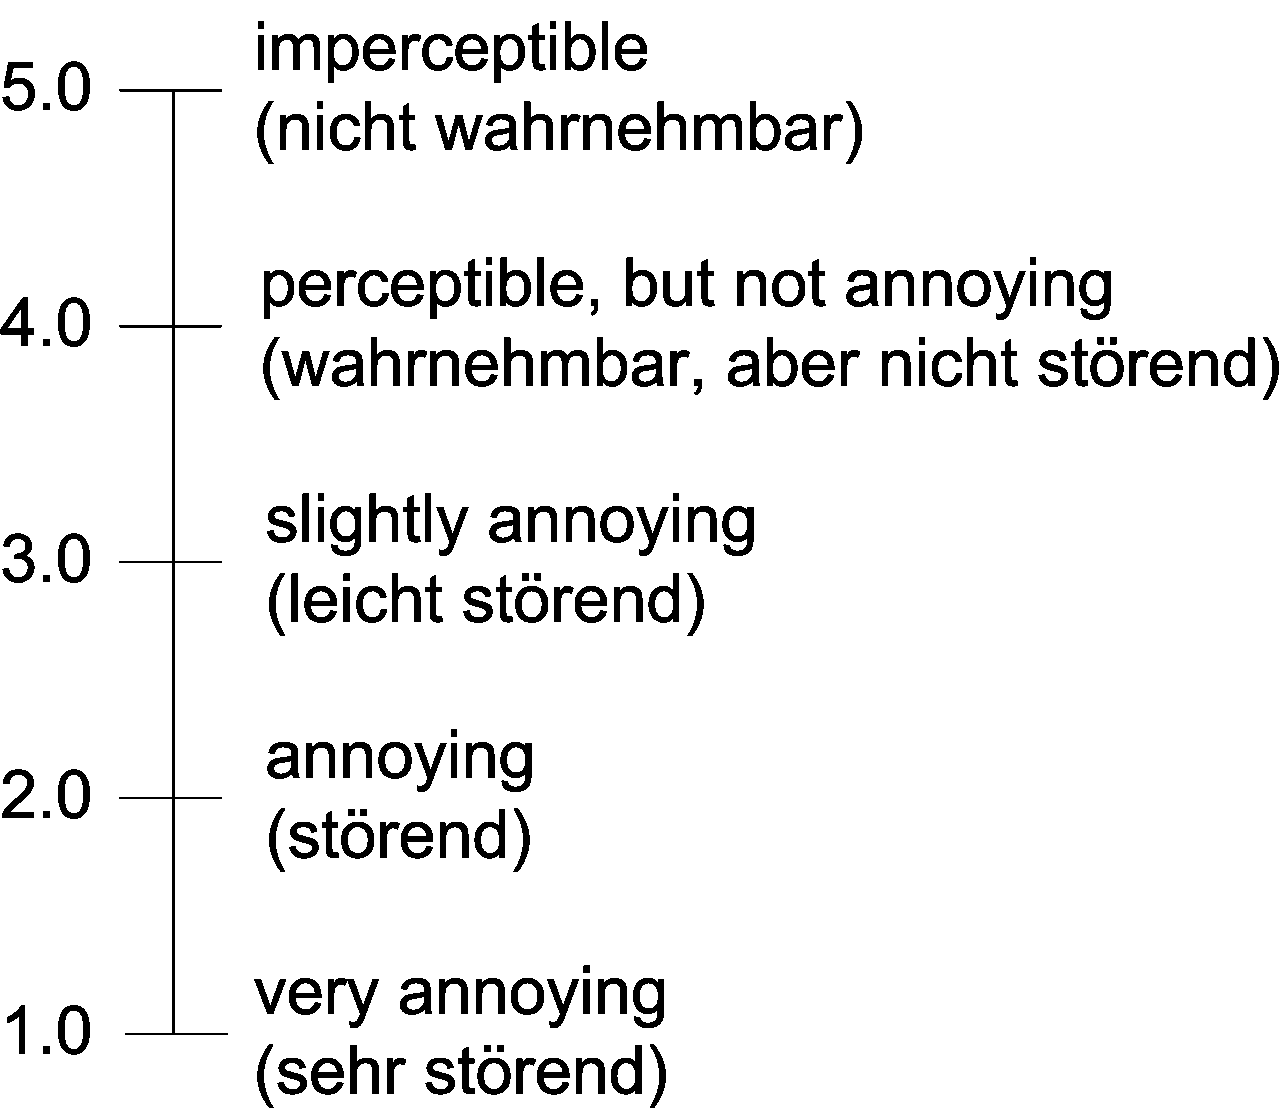
\includegraphics[scale=0.8]{graph/bewertungsscala}
			\end{figure}
			}
		\pause		
		example results
		\begin{table}
			\begin{center}
			\begin{footnotesize}
				\begin{tabular}{lccc}
				\hline
					\textbf{approach} & \textbf{SDG (app.)} \\
				\hline
				AAC/128, AC-3/192	& -0.5\\
				PAC/160	& -0.8\\
				PAC/128, AC-3/160, AAC/96, Layer 2/192	& -1.2 \ldots -1.0\\
				ITIS/192 	& -1.4\\
				Layer 3/128, Layer 2/160, PAC/96, ITIS/160 	& -1.8 \ldots -1.7\\
				AC-3/128, Layer 2/128, ITIS/128 	&  -2.2 \ldots -2.1\\
				PAC/64 	& -3.1\\
				ITIS/96 	& -3.3\\
				\end{tabular}  
			\end{footnotesize}
			\end{center}
		\end{table}
	\end{frame}		

\section{requirements}
	\begin{frame}{perceptual coding}{requirements}
        \begin{itemize}
            \item   quality (see above)
            \item	latency
                \begin{itemize}
                    \item   not important for file encoding, but for real-time transmission
                \end{itemize}
            \item	complexity
                \begin{itemize}
                    \item   encoder vs. decoder
                \end{itemize}
            \item   achievable bit rates
            \item   efficiency
                \begin{itemize}
                    \item   sound quality to bit rate
                \end{itemize}
            \item	availability and license
            \item   editability, scrolling capabilities
            \item   error resilience
		\end{itemize}
\end{frame}

\section{summary}
	\begin{frame}{perceptual coding}{summary}
        \begin{itemize}
            \item   perceptual codecs take advantage of properties of human hearing and combine this with principles of redundancy coding
            \item   (MPEG) encoders are only specified by their output stream $\Rightarrow$ different encoders have different quality
            \item   bitrate/quality tradeoff cannot be completely overcome, however, synthesis-based approaches  are more and more successful at low bitrates
		\end{itemize}
\end{frame}

\end{document}

